\chapter{Các fermion, ma trận Dirac và biển Dirac}

Biển Dirac là đích đến của chúng ta, nhưng con đường dẫn tới đó cũng quan trọng. Trước khi xét năng lượng âm trong lý thuyết electron tương đối tính, ta cần hai công cụ. Trước hết là đại số toán tử phân biệt fermion với boson. Tiếp theo là ôn lại phương trình Dirac một chiều, nơi có thể thấy rõ từng bước mở rộng hàm sóng mà không bị vướng vào hình học của ba chiều không gian. Khi đã có những công cụ ấy, phương trình ba chiều sẽ buộc ta phải có một cấu trúc ma trận riêng, và phần mở đầu bàn về các trạng thái fermion đầy và trống sẽ trở lại như chìa khóa để hiểu positron.

Ta dùng \(c=\hbar=1\). Chữ \(P\) viết hoa ký hiệu toán tử động lượng, chữ \(p\) viết thường ký hiệu trị riêng động lượng, còn các ký hiệu in đậm là phiên bản ba chiều của chúng.

\section{Trao đổi được biểu diễn bằng đại số toán tử}

Xét hai hạt giống hệt nhau, một hạt ở \(x\) và hạt kia ở \(y\). Các nhãn \(x\) và \(y\) chỉ các vị trí đầy đủ; chúng không phải là hai tọa độ Descartes của cùng một hạt. Tác dụng hai toán tử tạo lên chân không cho ta
\begin{equation}
\lvert x,y\rangle
=
\psi^\dagger(x)\psi^\dagger(y)\lvert0\rangle.
\label{eq:l10-two-particle-state}
\end{equation}

Đối với boson, đổi chỗ hai vị trí không làm thay đổi trạng thái:
\begin{equation}
\lvert x,y\rangle=\lvert y,x\rangle.
\end{equation}
Phát biểu toán tử bảo đảm tính đối xứng này là
\begin{equation}
\psi^\dagger(x)\psi^\dagger(y)
=
\psi^\dagger(y)\psi^\dagger(x).
\label{eq:l10-boson-exchange}
\end{equation}
Hai toán tử tạo boson giao hoán, nên ta có thể đảo thứ tự của chúng mà không làm thay đổi trạng thái được tạo ra.

Đối với fermion, phép đổi chỗ làm đổi dấu:
\begin{equation}
\lvert x,y\rangle=-\lvert y,x\rangle.
\label{eq:l10-fermion-state-exchange}
\end{equation}
Dấu tổng thể của một vectơ trạng thái riêng lẻ không phải là đại lượng quan sát được, nhưng dấu tương đối giữa các khả năng thì có thể quan sát được, vì vậy phải giữ nhất quán dấu trừ này. Phương trình~\eqref{eq:l10-fermion-state-exchange} đòi hỏi
\begin{equation}
\psi^\dagger(x)\psi^\dagger(y)
=
-\,\psi^\dagger(y)\psi^\dagger(x).
\label{eq:l10-fermion-operator-exchange}
\end{equation}

\begin{figure}[htbp]
\centering
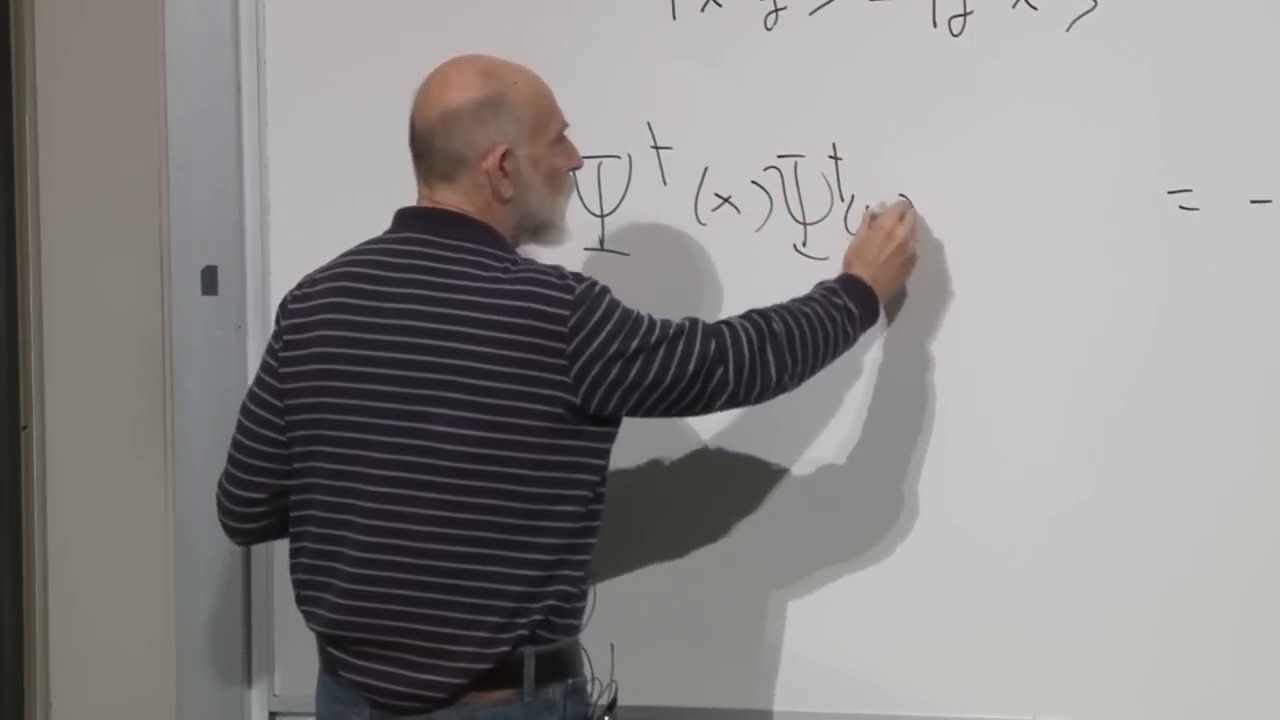
\includegraphics[width=0.94\linewidth]{lecture_10_figure_02.png}
\caption{Quan hệ trên bảng biểu diễn phép trao đổi fermion. Đổi chỗ các toán tử tạo làm đổi dấu trạng thái hai hạt.}
\lectureframe{00:05:50}
\end{figure}

Với hai toán tử bất kỳ \(A\) và \(B\), ta định nghĩa phản giao hoán tử là
\begin{equation}
\{A,B\}:=AB+BA.
\end{equation}
Do đó, quy tắc trao đổi là
\begin{equation}
\{\psi^\dagger(x),\psi^\dagger(y)\}=0.
\label{eq:l10-creation-anticommutator}
\end{equation}
Đại số trường fermion tương ứng thay các giao hoán tử của boson bằng phản giao hoán tử. Cần phân biệt hai cách dùng từ này: các toán tử trường phản giao hoán do thống kê Fermi, còn các ma trận sau này sẽ phản giao hoán để triệt tiêu các số hạng chéo trong hệ thức tán sắc tương đối tính.

Bây giờ đặt \(y=x\) trong Eq.~\eqref{eq:l10-creation-anticommutator}. Hai tích trở thành như nhau:
\begin{align}
0
&=\{\psi^\dagger(x),\psi^\dagger(x)\}\\
&=2\,\psi^\dagger(x)\psi^\dagger(x).
\end{align}
Vậy
\begin{equation}
\bigl(\psi^\dagger(x)\bigr)^2=0.
\label{eq:l10-exclusion}
\end{equation}
Cố tạo hai fermion giống hệt nhau trong cùng một trạng thái một hạt sẽ cho vectơ không. Đó là nguyên lý loại trừ ở dạng toán tử.

\begin{figure}[htbp]
\centering
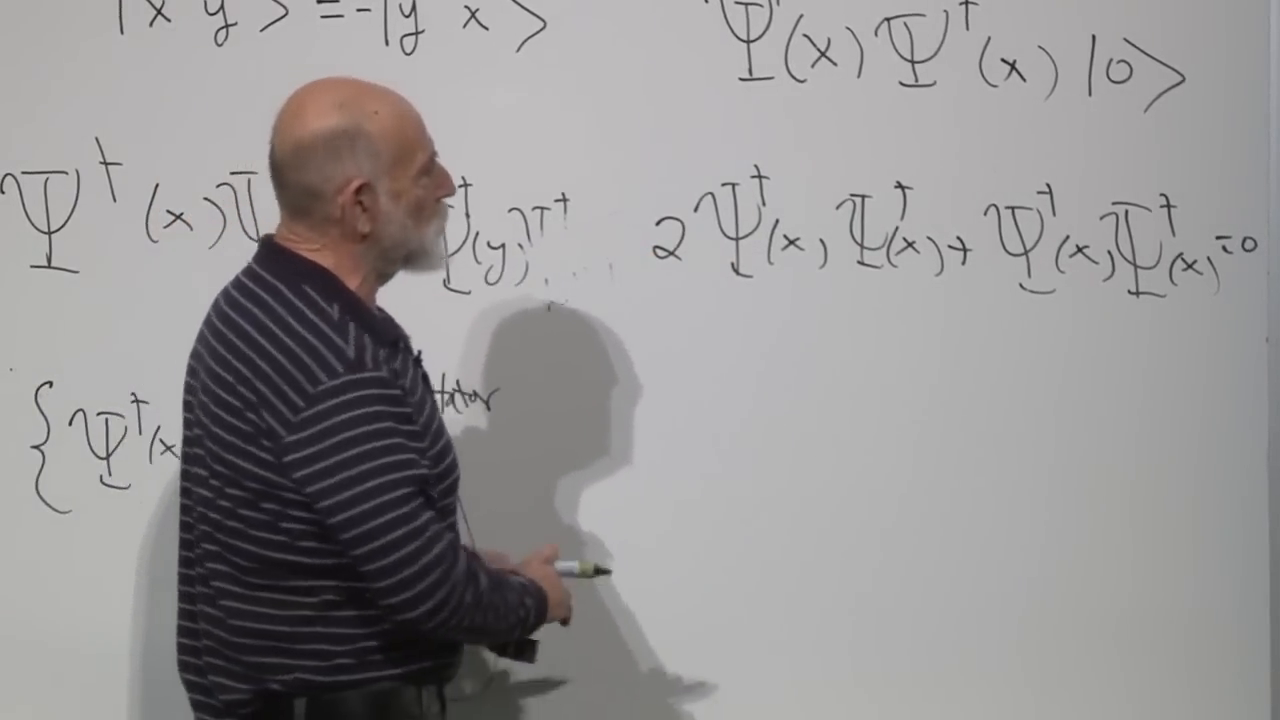
\includegraphics[width=0.94\linewidth]{lecture_10_figure_03.png}
\caption{Trường hợp hai trạng thái bằng nhau trên bảng. Tích lặp của các toán tử tạo xuất hiện hai lần nên phải triệt tiêu.}
\lectureframe{00:08:04}
\end{figure}

\begin{figure}[htbp]
\centering
\begin{adjustbox}{max width=\linewidth}
\begin{tikzpicture}[node distance=1.25cm,>=Latex]
\node[draw,rounded corners,align=center,inner sep=7pt] (a)
  {$\{\psi^\dagger(x),\psi^\dagger(x)\}=0$};
\node[draw,rounded corners,align=center,inner sep=7pt,right=of a] (b)
  {$2(\psi^\dagger(x))^2=0$};
\node[draw,rounded corners,align=center,inner sep=7pt,right=of b] (c)
  {$(\psi^\dagger(x))^2=0$};
\draw[->,thick] (a) -- (b);
\draw[->,thick] (b) -- (c);
\end{tikzpicture}
\end{adjustbox}
\caption{Lập luận về nguyên lý loại trừ được dựng lại đầy đủ, không có phần trung gian trên bảng đã bị xóa dở.}
\end{figure}

\section{Vì sao trạng thái đầy và trống đối xứng với nhau đối với fermion}

Có một khác biệt thứ hai giữa toán tử boson và fermion, tinh tế hơn nguyên lý loại trừ và về sau sẽ rất quan trọng. Với một mode boson,
\begin{equation}
[a,a^\dagger]=1,
\qquad
n=0,1,2,\ldots.
\end{equation}
Đổi thứ tự \(a\) và \(a^\dagger\) làm đổi dấu giao hoán tử. Ngay cả khi chỉ gọi các toán tử là \(A\) và \(B\), đại số vẫn cho ta biết thứ tự nào làm tăng số chiếm và thứ tự nào làm giảm nó.

Thang số chiếm của boson còn có một chiều xác định. Toán tử hủy cuối cùng đi tới \(\lvert0\rangle\) và tác dụng lên đó cho kết quả không, trong khi toán tử tạo có thể tiếp tục mãi:
\begin{align}
a\lvert0\rangle&=0,\\
a^\dagger\lvert n\rangle&\propto\lvert n+1\rangle,
\qquad n=0,1,2,\ldots.
\end{align}
Lật ngược thang này không cho lại cùng một phổ. Thang có đáy nhưng không có đỉnh.

Với một mode fermion,
\begin{equation}
\{a,a^\dagger\}=1,
\qquad
a^2=(a^\dagger)^2=0,
\qquad
n=0,1.
\label{eq:l10-fermion-mode}
\end{equation}
Toán tử tạo đưa trạng thái trống thành trạng thái đầy rồi dừng lại:
\begin{equation}
a^\dagger\lvert0\rangle=\lvert1\rangle,
\qquad
a^\dagger\lvert1\rangle=0.
\end{equation}
Toán tử hủy thực hiện quá trình ngược lại:
\begin{equation}
a\lvert1\rangle=\lvert0\rangle,
\qquad
a\lvert0\rangle=0.
\end{equation}
Chỉ có hai trạng thái, nên sơ đồ đối xứng khi đổi trạng thái đầy với trạng thái trống và đổi \(a\) với \(a^\dagger\). Các toán tử vẫn mang ý nghĩa vật lý khác nhau, nhưng đại số của chúng không còn ưu tiên toán tử này là toán tử tạo và toán tử kia là toán tử hủy. Sự đối xứng hình thức này là mầm mống của cách diễn giải lại theo hạt và lỗ trống.

\begin{classroomqa}
\lecturetimestamp{00:13:54}
\audiencequestion{Nếu \((a^\dagger)^2=0\), điều đó có mâu thuẫn không, hay nó hàm ý rằng \(a^\dagger=0\)?}
\lecturerresponse{Không phải cả hai. Một toán tử khác không có thể có bình phương bằng không. Ở đây, \(a^\dagger\) biến \(\lvert0\rangle\) thành \(\lvert1\rangle\), nhưng không có trạng thái khả dĩ nào phía trên \(\lvert1\rangle\), nên tác dụng toán tử ấy hai lần cho kết quả không. Lập luận tương tự cho ta \(a^2=0\).}
\end{classroomqa}

Hãy tạm ghi nhớ sự đối xứng giữa trạng thái đầy và trống này. Khi một electron năng lượng âm bị lấy đi, toán tử hủy sẽ được đổi tên thành toán tử tạo positron. Đó không phải là thay đổi ký hiệu tùy tiện; phép đổi tên này sử dụng đúng đại số fermion hai trạng thái đã thiết lập ở đây.

\section{Cấu tạo phương trình Dirac một chiều}

Giờ hãy trở lại với một hạt trong một chiều không gian. Phương trình sóng tương đối tính bậc nhất đơn giản nhất là
\begin{equation}
i\partial_t\psi=-\,i\partial_x\psi.
\label{eq:l10-right-mover}
\end{equation}
Với \(P=-i\partial_x\), ta có
\begin{equation}
H=P.
\end{equation}
Trạng thái riêng động lượng có \(E=p\), và vận tốc nhóm của nó là
\begin{equation}
v_g=\frac{dE}{dp}=1.
\end{equation}
Động lượng dương hay âm, và do đó năng lượng dương hay âm, vẫn cho một sóng truyền cứng sang phải. Dấu của \(p\) làm thay đổi dạng pha, chứ không làm đổi hướng truyền.

Một hạt có khối lượng phải có khả năng chuyển động theo cả hai hướng. Đưa vào thành phần thứ hai thỏa mãn
\begin{equation}
H\psi_1=P\psi_1,
\qquad
H\psi_2=-P\psi_2.
\label{eq:l10-two-directions}
\end{equation}
Thành phần thứ nhất truyền sang phải; thành phần thứ hai truyền sang trái. Gom chúng thành một cột,
\begin{equation}
\Psi=
\begin{pmatrix}
\psi_1\\
\psi_2
\end{pmatrix},
\end{equation}
và định nghĩa
\begin{equation}
\alpha=
\begin{pmatrix}
1&0\\
0&-1
\end{pmatrix}.
\end{equation}
Cả hai phương trình trở thành
\begin{equation}
H\Psi=\alpha P\Psi.
\label{eq:l10-massless-one-d}
\end{equation}
Cái giá phải trả để bao gồm cả hai hướng là một bậc tự do nội tại hai giá trị mới.

Chỉ riêng hướng chuyển động không tạo ra khối lượng. Đưa vào ma trận thứ hai,
\begin{equation}
\beta=
\begin{pmatrix}
0&1\\
1&0
\end{pmatrix},
\end{equation}
và thử
\begin{equation}
H=\alpha P+\beta m.
\label{eq:l10-massive-one-d}
\end{equation}
Các ma trận thỏa mãn
\begin{equation}
\alpha^2=\beta^2=\mathbb{1},
\qquad
\{\alpha,\beta\}=0.
\label{eq:l10-one-d-algebra}
\end{equation}
Bình phương Hamiltonian cho ta
\begin{align}
H^2
&=(\alpha P+\beta m)^2\\
&=\alpha^2P^2+\beta^2m^2
  +(\alpha\beta+\beta\alpha)Pm\\
&=P^2+m^2.
\label{eq:l10-one-d-dispersion}
\end{align}
Phản giao hoán tử trong Eq.~\eqref{eq:l10-one-d-algebra} loại bỏ số hạng không mong muốn tuyến tính theo cả \(P\) lẫn \(m\).

Ma trận ngoài đường chéo \(\beta\) ghép hai thành phần có hướng truyền khác nhau. Có thể hình dung số hạng khối lượng liên tục trộn các biên độ truyền sang phải và truyền sang trái. Không nên hiểu hình dung này theo nghĩa đen rằng hạt nảy qua lại trên một đường vi mô, nhưng nó giúp nắm được vì sao gói sóng có khối lượng có thể có tốc độ trung bình nhỏ hơn tốc độ ánh sáng và có thể có hệ quy chiếu nghỉ, trong khi một thành phần chiral không khối lượng cô lập thì không thể.

\begin{classroomqa}
\lecturetimestamp{00:23:37}
\audiencequestion{Việc đưa vào cả hai thành phần có cách diễn giải vật lý sâu hơn nào không?}
\lecturerresponse{Có, nhưng cách diễn giải ấy sẽ hiện rõ hơn trong ba chiều. Ở giai đoạn này, chúng đơn thuần là hai thành phần cần có để mô tả hai hướng truyền ngược nhau và cho phép có ghép khối lượng ngoài đường chéo. Cách diễn giải về sau là tính thuận tay, hay tính chiral.}
\end{classroomqa}

\section{Ba chiều buộc ta phải dùng ma trận Pauli}

Trong ba chiều không gian, động lượng là một vectơ. Một Hamiltonian tuyến tính theo động lượng và là vô hướng dưới phép quay gợi ý cần có một vectơ khác, lần này là vectơ có các thành phần là ma trận:
\begin{equation}
H=\boldsymbol{\alpha}\cdot\mathbf P
=\alpha_xP_x+\alpha_yP_y+\alpha_zP_z.
\label{eq:l10-three-d-ansatz}
\end{equation}

\begin{figure}[htbp]
\centering
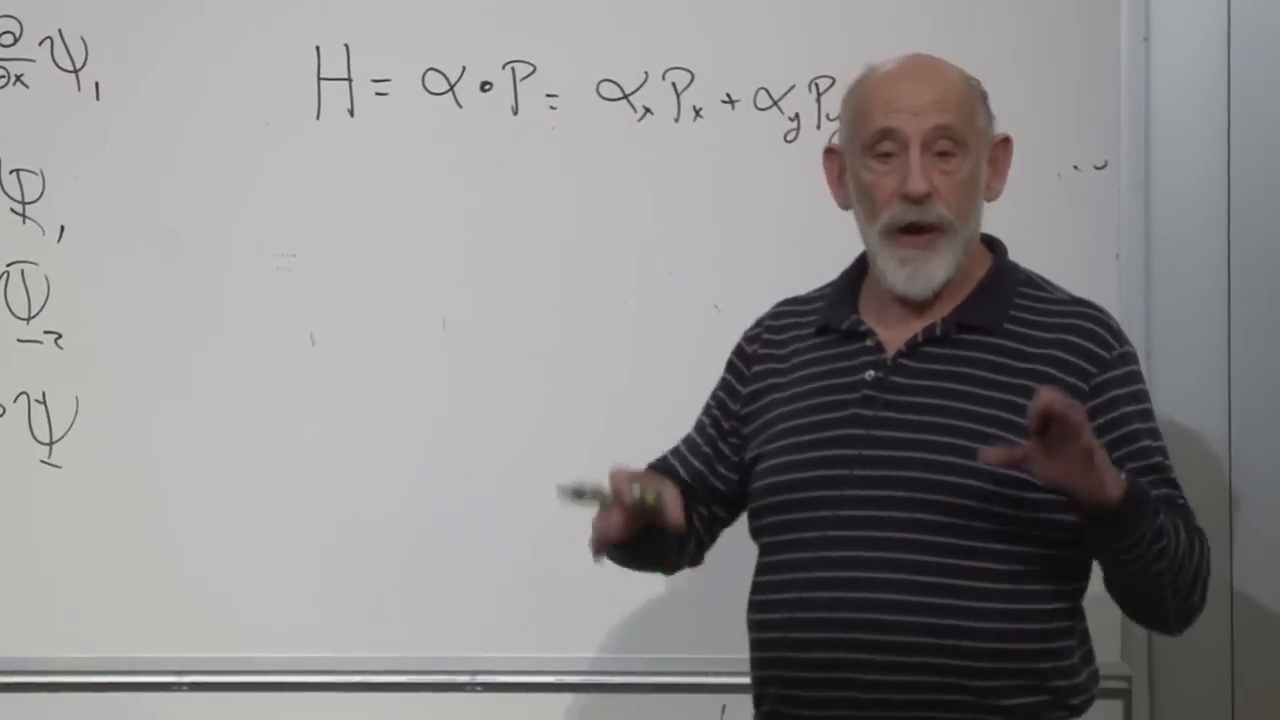
\includegraphics[width=0.94\linewidth]{lecture_10_figure_04.png}
\caption{Dạng giả thiết không khối lượng ba chiều \(H=\boldsymbol{\alpha}\cdot\mathbf P\) tại thời điểm một ma trận được mở rộng thành một vectơ gồm ba ma trận.}
\lectureframe{00:26:00}
\end{figure}

Bắt đầu lại với trường hợp không khối lượng. Ta yêu cầu
\begin{equation}
H^2=\mathbf P^2=P_x^2+P_y^2+P_z^2.
\end{equation}
Khai triển bình phương của Eq.~\eqref{eq:l10-three-d-ansatz},
\begin{align}
H^2
&=\alpha_x^2P_x^2+\alpha_y^2P_y^2\\
&\quad+\alpha_z^2P_z^2\\
&\quad+\{\alpha_x,\alpha_y\}P_xP_y\\
&\quad+\{\alpha_x,\alpha_z\}P_xP_z\\
&\quad+\{\alpha_y,\alpha_z\}P_yP_z.
\end{align}
Các số hạng đường chéo có dạng đúng nếu
\begin{equation}
\alpha_x^2=\alpha_y^2=\alpha_z^2=\mathbb{1},
\end{equation}
và mọi số hạng chéo triệt tiêu nếu
\begin{equation}
\{\alpha_i,\alpha_j\}=0,
\qquad i\ne j.
\label{eq:l10-alpha-anticommutation}
\end{equation}

Ba ma trận \(2\times2\) quen thuộc thực hiện đúng điều này:
\begin{equation}
\sigma_x=
\begin{pmatrix}
0&1\\
1&0
\end{pmatrix},
\quad
\sigma_y=
\begin{pmatrix}
0&-i\\
i&0
\end{pmatrix},
\quad
\sigma_z=
\begin{pmatrix}
1&0\\
0&-1
\end{pmatrix}.
\label{eq:l10-pauli-matrices}
\end{equation}
Vậy một nghiệm là
\begin{equation}
\alpha_i=\sigma_i,
\qquad
H=\boldsymbol{\sigma}\cdot\mathbf P.
\label{eq:l10-weyl-hamiltonian}
\end{equation}

\begin{figure}[htbp]
\centering
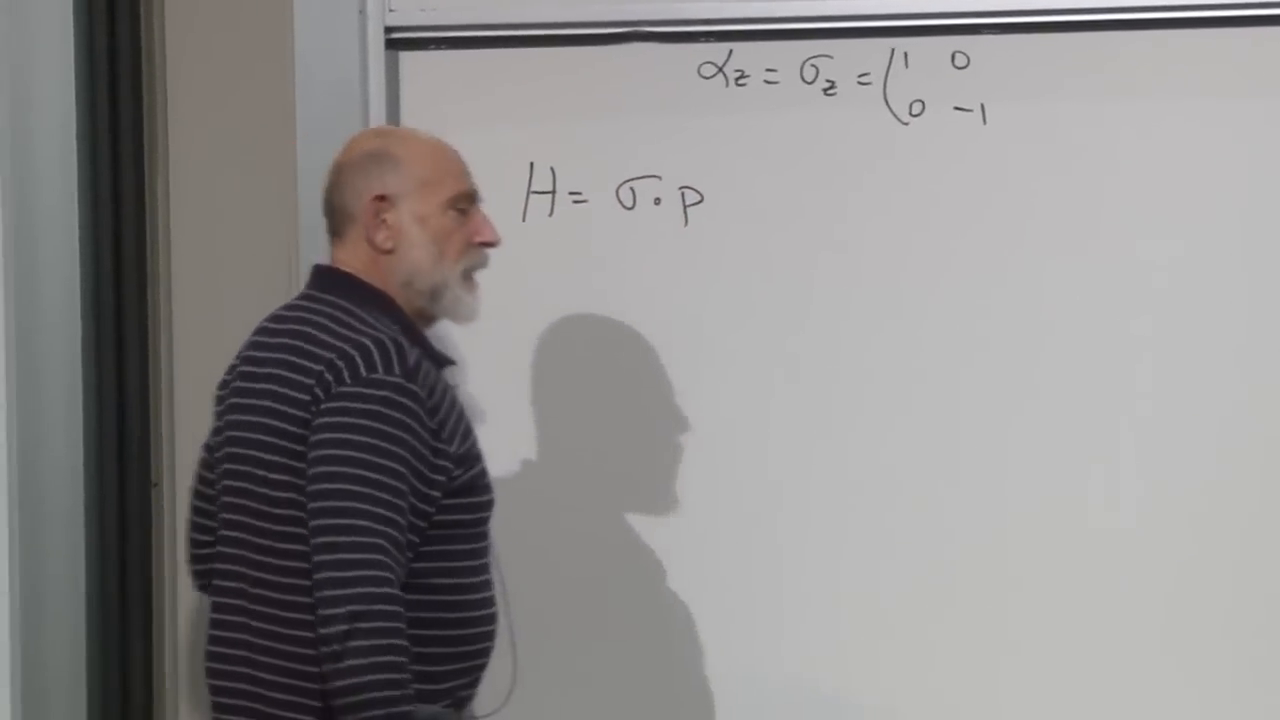
\includegraphics[width=0.94\linewidth]{lecture_10_figure_05.png}
\caption{Hamiltonian không khối lượng dạng gọn \(H=\boldsymbol{\sigma}\cdot\mathbf P\), với \(\alpha_z=\sigma_z\) vẫn được ghi rõ phía trên.}
\lectureframe{00:28:16}
\end{figure}

Với một trạng thái riêng động lượng,
\begin{equation}
\boldsymbol{\sigma}\cdot\mathbf p
=
|\mathbf p|\,\boldsymbol{\sigma}\cdot\widehat{\mathbf p}.
\end{equation}
Toán tử \(\boldsymbol{\sigma}\cdot\widehat{\mathbf p}\) có các trị riêng \(+1\) và \(-1\), nên
\begin{equation}
E=\pm|\mathbf p|.
\end{equation}
Trong lý thuyết hai thành phần này, với năng lượng dương, bậc tự do Pauli định hướng song song với động lượng; với năng lượng âm, nó định hướng ngược chiều. Hướng này bị ràng buộc, chứ không phải là hướng spin có thể điều chỉnh độc lập khi dấu năng lượng đã cố định.

\begin{classroomqa}
\lecturetimestamp{00:30:10}
\audiencequestion{Spin có tự xuất hiện từ phương trình Dirac không, hay được đưa vào vì ta đã biết electron có mômen từ?}
\lecturerresponse{Ở đây, “tự xuất hiện” có nghĩa là “suy ra như một hệ quả”, chứ không phải “biến mất”. Điểm xuất phát là yêu cầu một Hamiltonian tuyến tính theo động lượng, có bình phương bằng \(\mathbf P^2\). Các số thông thường không thể thỏa mãn đại số cần thiết, nhưng ma trận Pauli thì có thể. Vì vậy, cấu trúc hai thành phần của chúng xuất hiện ngay trong quá trình tuyến tính hóa. Điều này không chứng minh rằng hạt nào cũng phải có spin; nó chỉ nói rằng các hạt được mô tả bằng phương trình kiểu Dirac này mang bậc tự do spinor tương ứng.}
\end{classroomqa}

Đây là một trong những bài học cốt lõi của phép dựng này. Các ma trận không phải những nhãn trang trí được thêm vào sau khi tìm ra phương trình tương đối tính. Chính nỗ lực lấy căn bậc hai địa phương của hệ thức tán sắc tương đối tính đã dẫn đến chúng.

\section{Vì sao khối lượng đòi hỏi bốn thành phần}

Hãy thử lặp lại phép dựng khối lượng một chiều mà không mở rộng lý thuyết \(2\times2\):
\begin{equation}
H=\boldsymbol{\sigma}\cdot\mathbf P+\beta m.
\label{eq:l10-failed-mass}
\end{equation}
Giả sử \(\beta^2=\mathbb{1}\). Bình phương chứa các số hạng mong muốn \(\mathbf P^2+m^2\), nhưng còn có cả
\begin{equation}
m\sum_i\{\sigma_i,\beta\}P_i.
\end{equation}
Để loại bỏ số hạng này, một ma trận \(\beta\) phải thỏa mãn
\begin{equation}
\{\sigma_x,\beta\}
=
\{\sigma_y,\beta\}
=
\{\sigma_z,\beta\}
=0.
\label{eq:l10-impossible-beta}
\end{equation}
Không có ma trận \(2\times2\) nào làm được điều đó. Ma trận đơn vị giao hoán với cả ba ma trận Pauli, còn mọi ma trận \(2\times2\) không vết đều là tổ hợp tuyến tính của các ma trận Pauli. Bất kỳ tổ hợp nào như vậy cũng không phản giao hoán với thành phần song song với nó. Đại số \(2\times2\) không có ma trận độc lập thứ tư với tính chất cần thiết.

Giải pháp là mở rộng spinor. Bốn ma trận phản giao hoán đôi một và có bình phương bằng ma trận đơn vị chỉ xuất hiện lần đầu trong một biểu diễn phức \(4\times4\). Không chọn kích thước ma trận này vì không-thời gian có bốn chiều; đây là không gian ma trận nhỏ nhất có thể hiện thực hóa đại số cần thiết.

Có nhiều biểu diễn tương đương. Phép đổi cơ sở đơn nhất của spinor làm thay đổi các phần tử của mọi ma trận mà không làm thay đổi bất kỳ dự đoán vật lý nào. Điều quan trọng là tập hợp các hệ thức trừu tượng
\begin{equation}
\{\alpha_i,\alpha_j\}=2\delta_{ij}\mathbb{1},
\qquad
\{\alpha_i,\beta\}=0,
\qquad
\beta^2=\mathbb{1}.
\label{eq:l10-dirac-algebra}
\end{equation}

\begin{classroomqa}
\lecturetimestamp{00:37:38}
\audiencequestion{Có thể xem \(\beta\) là thành phần thời gian \(\alpha_t\) không?}
\lecturerresponse{Không thể làm vậy một cách trực tiếp. Ba ma trận \(\alpha_i\) không hợp với \(\beta\) thành bốn thành phần của một vectơ Lorentz duy nhất. Thay vào đó, trong ký hiệu hiệp biến, ta định nghĩa \(\beta=\gamma^0\) và \(\alpha_i=\gamma^0\gamma^i\); bốn ma trận \(\gamma^\mu\) thỏa mãn đại số Clifford của không-thời gian.}
\end{classroomqa}

Một biểu diễn khối thuận tiện là
\begin{equation}
\alpha_i=
\begin{pmatrix}
\sigma_i&0\\
0&-\sigma_i
\end{pmatrix},
\qquad
\beta=
\begin{pmatrix}
0&I_2\\
I_2&0
\end{pmatrix}.
\label{eq:l10-block-representation}
\end{equation}
Các ma trận Pauli trong các khối đường chéo bảo đảm các \(\alpha_i\) phản giao hoán đôi một. Các khối đơn vị ngoài đường chéo trong \(\beta\) bảo đảm \(\beta\) phản giao hoán với mọi \(\alpha_i\).

\begin{figure}[htbp]
\centering
\includegraphics[width=0.94\linewidth]{lecture_10_figure_06.png}
\caption{Biểu diễn khối \(4\times4\) trên bảng. Các phương trình phía trên ghi lại các phản giao hoán tử cần có; toàn bộ ma trận được viết thành ký hiệu trong Eq.~\eqref{eq:l10-block-representation}.}
\lectureframe{00:41:10}
\end{figure}

Giờ đây Hamiltonian có khối lượng là
\begin{equation}
H=\boldsymbol{\alpha}\cdot\mathbf P+\beta m
=
\begin{pmatrix}
\boldsymbol{\sigma}\cdot\mathbf P&mI_2\\
mI_2&-\boldsymbol{\sigma}\cdot\mathbf P
\end{pmatrix}.
\label{eq:l10-massive-dirac}
\end{equation}
Dùng Eq.~\eqref{eq:l10-dirac-algebra},
\begin{equation}
H^2=\mathbf P^2+m^2.
\end{equation}
Vì vậy, cấu trúc bốn thành phần không phải phần bổ sung tùy chọn. Đó là cấu trúc nhỏ nhất cho phép đồng thời có động lượng ba chiều và số hạng khối lượng mà vẫn giữ phương trình ở bậc nhất.

\section{Tính chiral và ý nghĩa của các thành phần bổ sung}

Phép mở rộng đã bổ sung khác biệt vật lý nào? Hãy bắt đầu với khối trên không khối lượng,
\begin{equation}
H_R=\boldsymbol{\sigma}\cdot\mathbf P,
\end{equation}
và khối dưới không khối lượng,
\begin{equation}
H_L=-\boldsymbol{\sigma}\cdot\mathbf P.
\end{equation}
Đối với các trạng thái năng lượng dương, spin của khối thứ nhất song song với động lượng, còn spin của khối thứ hai ngược chiều với động lượng. Đó là hai độ xoắn đối nhau. Trong lý thuyết không khối lượng, độ xoắn bất biến dưới các phép biến đổi Lorentz chính tắc, vì không quan sát viên nào có thể vượt một hạt chuyển động như ánh sáng rồi đảo chiều động lượng của nó mà vẫn giữ nguyên spin. Do đó, hai khối mô tả hai khu vực chiral đối nhau.

\begin{classroomqa}
\lecturetimestamp{00:41:28}
\audiencequestion{Trong một chiều, cần thêm một bậc tự do nhị phân để đưa khối lượng vào. Trong ba chiều, khác biệt vật lý tương ứng là gì?}
\lecturerresponse{Đó là tính thuận tay của spinor. Hai khối \(2\times2\) có quan hệ giữa spin và động lượng ngược nhau. Một khối thuận tay phải, khối kia thuận tay trái. Lý thuyết \(4\times4\) chứa cả hai.}
\end{classroomqa}

Số hạng khối lượng trong Eq.~\eqref{eq:l10-massive-dirac} nằm ngoài đường chéo. Nó chuyển biên độ của khối trên sang khối dưới và ngược lại:
\begin{equation}
\beta m
\begin{pmatrix}
\Psi_R\\
\Psi_L
\end{pmatrix}
=
m
\begin{pmatrix}
\Psi_L\\
\Psi_R
\end{pmatrix}.
\end{equation}
Vì vậy, khối lượng là sự ghép nối giữa hai tính chiral đối nhau.

\begin{classroomqa}
\lecturetimestamp{00:43:58}
\audiencequestion{Một hạt không khối lượng có thể đổi tính chiral không?}
\lecturerresponse{Không, với Hamiltonian tự do không khối lượng được trình bày ở đây. Hai khối không ghép với nhau, nên trạng thái ban đầu thuận tay phải hoặc trái sẽ giữ nguyên như vậy. Chính số hạng khối lượng ngoài đường chéo làm trộn chúng khi \(m\ne0\).}
\end{classroomqa}

Cách diễn đạt này chính xác đối với biểu diễn khối, nhưng không nên đẩy quá xa hình ảnh một hạt lật cơ học qua lại giữa hai mũi tên. Phát biểu vật lý ở đây là sự ghép nối ma trận trong phương trình sóng.

\begin{classroomqa}
\lecturetimestamp{00:44:50}
\audiencequestion{Các ma trận này có được hàm chứa trong quaternion không?}
\lecturerresponse{Các ma trận Pauli có liên hệ chặt chẽ với các đơn vị quaternion: bình phương của các ma trận \(-i\sigma_i\) bằng \(-\mathbb{1}\) và phép nhân của chúng tuân theo quy tắc quaternion, tùy theo quy ước định hướng. Các ma trận Dirac đầy đủ đòi hỏi đại số Clifford lớn hơn, và không cần đến mối liên hệ với quaternion cho lập luận tiếp theo.}
\end{classroomqa}

\begin{classroomqa}
\lecturetimestamp{00:46:34}
\audiencequestion{Nếu spin là mômen động lượng, ở đây có số hạng năng lượng riêng nào gắn với nó không?}
\lecturerresponse{Không có số hạng hạt tự do độc lập nào được thêm vào. Cấu trúc spinor đã đi vào Hamiltonian động năng thông qua các ma trận. Ghép spin với một từ trường ngoài sẽ đưa thêm các số hạng tương tác, nhưng đó là một bài toán khác.}
\end{classroomqa}

\section{Các ma trận alpha biểu diễn vận tốc, không phải spin}

Mỗi \(\alpha_i\) có hai trị riêng \(+1\) và hai trị riêng \(-1\). Các thành phần khác nhau không giao hoán, nên không thể đồng thời đo chính xác tất cả chúng. Để xác định một thành phần biểu diễn đại lượng nào, hãy dùng phương trình Heisenberg. Với toán tử \(L\) không phụ thuộc tường minh vào thời gian,
\begin{equation}
\dot L=i[H,L].
\label{eq:l10-heisenberg}
\end{equation}
Quy ước dấu ở đây được xác định theo sự tiến hóa Schr\"odinger \(e^{-iHt}\).

Áp dụng Eq.~\eqref{eq:l10-heisenberg} cho toán tử vị trí \(x\). Các ma trận tác dụng lên các chỉ số spinor và giao hoán với vị trí, trong khi chỉ có \(P_x\) không giao hoán với \(x\):
\begin{align}
\dot x
&=i[\boldsymbol{\alpha}\cdot\mathbf P+\beta m,x]\\
&=i\alpha_x[P_x,x]\\
&=\alpha_x,
\label{eq:l10-velocity}
\end{align}
vì \([P_x,x]=-i\). Do đó, \(\alpha_x\) là thành phần \(x\) của toán tử vận tốc; tương tự,
\begin{equation}
\dot{\mathbf x}=\boldsymbol{\alpha}.
\end{equation}

\begin{classroomqa}
\lecturetimestamp{00:51:50}
\audiencequestion{Phép đo một thành phần vận tốc có thực sự chỉ cho kết quả \(+1\) hoặc \(-1\) không?}
\lecturerresponse{Có, đối với toán tử tức thời \(\alpha_i\) trong đơn vị \(c=1\). Một trạng thái tổng quát không nhất thiết là trạng thái riêng, nên giá trị kỳ vọng của nó có thể nằm ở bất kỳ đâu giữa hai giá trị ấy. Gói sóng được truyền đi một cách liên tục có vận tốc trung bình nhỏ hơn tốc độ ánh sáng khi hạt có khối lượng.}
\end{classroomqa}

Vận tốc không được bảo toàn:
\begin{equation}
\dot\alpha_x=i[H,\alpha_x]\ne0.
\end{equation}
Các số hạng chứa \(\alpha_y\), \(\alpha_z\) và \(\beta\) không giao hoán với \(\alpha_x\). Vì vậy, trạng thái gồm cả thành phần năng lượng dương lẫn âm sẽ biểu hiện một đóng góp dao động nhanh trong vị trí. Hiện tượng này là \emph{chuyển động run}, nghĩa đen là chuyển động rung lắc.

Sau khi lấy trung bình trên khoảng thời gian dài hơn nhiều so với chu kỳ dao động nhanh, vận tốc tương đối tính kỳ vọng là
\begin{equation}
\overline{\mathbf v}=\frac{\mathbf p}{E},
\end{equation}
Với electron chuyển động chậm, biểu thức này rút gọn thành \(\mathbf p/m\).

\begin{classroomqa}
\lecturetimestamp{00:54:40}
\audiencequestion{Electron tự do run mà không chịu lực ngoài thì có vi phạm định luật Newton không?}
\lecturerresponse{Không. Tính bất biến tịnh tiến bảo toàn động lượng, nên \(\dot{\mathbf P}=0\). Toán tử vận tốc Dirac không đơn giản là \(\mathbf P/m\), và thành phần dao động nhanh của nó có thể thay đổi trong khi động lượng vẫn không đổi. Chuyển động lấy trung bình theo thời gian tuân theo hệ thức hạt tự do như dự kiến.}
\end{classroomqa}

\begin{classroomqa}
\lecturetimestamp{00:55:22}
\audiencequestion{Vận tốc có luôn bằng \(c\) không?}
\lecturerresponse{Phép đo tức thời của một \(\alpha_i\) có các trị riêng \(\pm c\), nhưng gói sóng có khối lượng nói chung là một chồng chập và có giá trị kỳ vọng dưới tốc độ ánh sáng. Vận tốc nhóm trung bình của nó là \(\mathbf p/E\).}
\end{classroomqa}

\begin{classroomqa}
\lecturetimestamp{00:55:30}
\audiencequestion{Có thể hình dung dao động này là do khối lượng làm vận tốc biến đổi không?}
\lecturerresponse{Không. Khối lượng là một tham số cố định. Dao động phát sinh từ các toán tử vận tốc và Hamiltonian không giao hoán, hay tương đương từ sự giao thoa giữa các vùng năng lượng, chứ không phải do khối lượng dao động.}
\end{classroomqa}

\begin{classroomqa}
\lecturetimestamp{00:56:22}
\audiencequestion{Phép đo tức thời có thể cho thấy vận tốc hướng theo một chiều, ngay cả khi chuyển động trung bình hướng theo chiều khác không?}
\lecturerresponse{Có. Toán tử thành phần có hai trị riêng xác định, còn các phép đo lặp lại hoặc lấy trung bình theo thời gian cho ta độ trôi liên tục hơn.}
\end{classroomqa}

Cũng cần dùng từ spin một cách cẩn trọng. Các \(\alpha_i\) biến đổi như những thành phần của vận tốc, một vectơ thông thường. Toán tử spin thực sự trong biểu diễn này là
\begin{equation}
\mathbf S=\frac12\boldsymbol{\Sigma},
\qquad
\Sigma_i=
\begin{pmatrix}
\sigma_i&0\\
0&\sigma_i
\end{pmatrix}.
\label{eq:l10-spin-operator}
\end{equation}
Nó khác \(\alpha_i\) ở dấu của khối dưới. Các ma trận có liên hệ chặt chẽ với nhau, nhưng vận tốc và spin không phải cùng một đại lượng quan sát được.

\section{Năng lượng âm và chân không có năng lượng thấp nhất}

Vấn đề năng lượng âm đã xuất hiện ngay cả trước khi có toàn bộ bộ máy ma trận này. Hãy trở lại với sóng truyền sang phải một chiều,
\begin{equation}
H=P.
\end{equation}
Vì \(p\) chạy trên toàn bộ trục số thực nên \(E=p\) không bị chặn dưới.

Chân không không thể chỉ có nghĩa là trạng thái không có hạt. Nó phải là trạng thái mà từ đó không thể lấy thêm năng lượng ra. Nếu trong trạng thái trống, ta có thể thêm một hạt năng lượng âm để hạ năng lượng, rồi thêm hạt khác và cứ tiếp tục vô hạn, thì trạng thái trống ấy không phải là chân không bền vững.

Thống kê Fermi đưa ra một lối thoát mang tính lịch sử. Đặt một electron vào mỗi trạng thái năng lượng âm. Mỗi electron được thêm vào làm giảm tổng năng lượng, nhưng nguyên lý loại trừ chỉ cho phép một electron trong mỗi trạng thái một hạt. Khi mọi trạng thái năng lượng âm đã đầy, không electron nào khác có thể rơi vào vùng ấy. Dirac đồng nhất cấu hình đầy này với chân không.

Cách dựng tương tự sẽ thất bại đối với boson. Một trạng thái có thể chứa số boson tùy ý, nên một mode boson năng lượng âm có thể hấp thụ hạt không giới hạn. Giới hạn fermion \(n=0,1\) được giới thiệu ở đầu bài giảng chính là điều ngăn năng lượng tiếp tục giảm mãi.

\begin{figure}[htbp]
\centering
\includegraphics[width=0.94\linewidth]{lecture_10_figure_07.png}
\caption{Hình ảnh biển Dirac mang tính lịch sử trên bảng: một thang các mức năng lượng âm được lấp đầy tới đường phân chia, bên trên là các trạng thái năng lượng dương.}
\lectureframe{01:02:45}
\end{figure}

\begin{figure}[htbp]
\centering
\begin{adjustbox}{max width=\linewidth}
\begin{tikzpicture}[x=1.05cm,y=0.72cm,>=Latex]
\draw[->] (0,-4.8) -- (0,4.8) node[above] {$E$};
\draw[thick] (-2.9,0) -- (3.2,0) node[right] {$E=0$};
\foreach \y in {-4,-3.3,...,-0.5} {
  \draw (-2.3,\y) -- (2.3,\y);
  \foreach \x in {-1.8,-1.2,...,1.8} {
    \fill[blue!65!black] (\x,\y) circle (1.6pt);
  }
}
\foreach \y in {0.8,1.6,...,4.0} {
  \draw (-2.3,\y) -- (2.3,\y);
}
\draw[red,very thick] (0.6,-2.6) circle (5pt);
\draw[red,->,very thick] (0.6,-2.35) .. controls (1.4,-0.4) and (1.2,1.6) .. (1.5,2.4);
\fill[red] (1.5,2.4) circle (2.5pt);
\node[right,red] at (0.85,-2.6) {hole};
\node[right,red] at (1.7,2.4) {$e^-$};
\node[left] at (-2.5,-2.2) {filled negative-energy states};
\end{tikzpicture}
\end{adjustbox}
\caption{Bản dựng lại rõ ràng về kích thích phía trên biển đầy: đưa một electron năng lượng âm lên cao hơn để lại một lỗ trống năng lượng dương.}
\end{figure}

Hình ảnh biển là cách diễn đạt mang tính lịch sử cho một phép sắp xếp lại toán tử đúng đắn. Không nên nhầm điện tích và năng lượng vô hạn của nó theo nghĩa đen với những đại lượng quan sát được trực tiếp; cách trình bày hiện đại sẽ loại bỏ nhu cầu hình dung electron vật chất lấp đầy không gian.

\section{Lỗ trống là positron}

Khi mọi trạng thái năng lượng âm đều đã bị chiếm, có thể tạo ra hai loại kích thích. Ta có thể thêm một electron năng lượng dương phía trên biển. Hoặc ta có thể lấy đi một electron năng lượng âm và để lại một lỗ trống.

Lỗ trống mang điện tích ngược dấu với electron bị thiếu. Lấy đi điện tích \(-e\) làm điện tích thay đổi một lượng \(+e\). Lỗ trống cũng có năng lượng kích thích dương. Nếu electron bị lấy đi có \(E_-<0\), thì năng lượng đo tương đối với chân không đầy thay đổi một lượng
\begin{equation}
E_{\mathrm{hole}}=-E_->0.
\end{equation}
Lỗ trống là một kích thích có năng lượng dương và điện tích dương: positron.

Một photon có thể kích thích electron trong biển lên một trạng thái năng lượng dương. So với chân không, trạng thái cuối chứa một electron và một positron. Trong giản đồ có thứ tự thời gian, theo quy ước ta vẽ dòng số electron hướng lên đối với electron, còn đường biểu diễn positron có mũi tên ngược chiều. Các mũi tên biểu thị dòng số fermion hoặc dòng điện tích; chúng không phải những vectơ vận tốc cổ điển nhỏ bé.

\begin{classroomqa}
\lecturetimestamp{01:05:14}
\audiencequestion{Hình ảnh này có đòi hỏi số electron và positron bằng nhau không?}
\lecturerresponse{Không phải trong một trạng thái bất kỳ. Bắt đầu từ chân không và tạo một cặp trung hòa thì có một hạt mỗi loại, nhưng một trạng thái có thể vốn đã chứa số electron dư hoặc số positron dư. Bảo toàn điện tích ràng buộc các phản ứng; nó không đòi hỏi mọi trạng thái khả dĩ phải có số lượng hai loại hạt bằng nhau.}
\end{classroomqa}

Ban đầu Dirac chưa biết rằng lỗ trống sẽ là một hạt có khối lượng bằng khối lượng electron và chỉ khác về điện tích cùng các số lượng tử cộng tính khác. Phương trình và phép dựng lỗ trống đã dẫn đến dự đoán ấy trước khi positron được đưa vào danh mục hạt quen thuộc.

\section{Một trường fermion chứa cả electron lẫn positron}

Toán tử trường đưa hình ảnh mang tính lịch sử này vào đại số hiện đại. Tạm thời bỏ qua các chỉ số spinor, hệ số chuẩn hóa và sự phụ thuộc thời gian. Một trường một chiều có thể được khai triển dưới dạng sơ đồ như sau:
\begin{equation}
\psi(x)
\sim
\int_{-\infty}^{\infty}dp\,a(p)e^{ipx}.
\label{eq:l10-full-field-integral}
\end{equation}
Với hệ thức tán sắc của sóng truyền sang phải \(E=p\), \(p\) dương ứng với năng lượng dương, còn \(p\) âm ứng với năng lượng âm. Tách tích phân:
\begin{equation}
\psi(x)
\sim
\int_0^\infty dp\,a(p)e^{ipx}
+
\int_{-\infty}^0 dp\,a(p)e^{ipx}.
\end{equation}
Trong số hạng thứ hai, đặt \(p=-q\), với \(q>0\), rồi diễn giải lại phép hủy electron năng lượng âm trong trạng thái đầy thành phép tạo positron:
\begin{equation}
b^\dagger(q):=a(-q).
\end{equation}
Khi đó
\begin{equation}
\psi(x)
\sim
\int_0^\infty dp\,
\left[
a(p)e^{ipx}
+
b^\dagger(p)e^{-ipx}
\right].
\label{eq:l10-electron-positron-split}
\end{equation}
Dấu chính xác của các pha sóng phẳng phụ thuộc vào quy ước không-thời gian; nội dung bất biến là \(\psi\) chứa một toán tử hủy electron và một toán tử tạo positron.

\begin{figure}[htbp]
\centering
\includegraphics[width=0.94\linewidth]{lecture_10_figure_08.png}
\caption{Tích phân trường được tách thành các vùng năng lượng dương và âm. Dòng dưới đổi nhãn toán tử electron năng lượng âm thành toán tử tạo positron.}
\lectureframe{01:11:35}
\end{figure}

Đây là lúc sự đối xứng giữa trạng thái đầy và trống trong Eq.~\eqref{eq:l10-fermion-mode} phát huy tác dụng. Đối với fermion, đại số toán tử cho phép đổi nhãn như vậy mà không làm thay đổi cấu trúc phản giao hoán.

Một tương tác điện từ dạng sơ đồ có dạng
\begin{equation}
H_{\mathrm{int}}
\sim
\int dx\,\psi^\dagger(x)\psi(x)A(x),
\label{eq:l10-qed-schematic}
\end{equation}
trong đó \(A\) ký hiệu trường photon. Vì mỗi trường fermion đều chứa các thành phần electron và positron, một toán tử địa phương duy nhất chứa một số kênh:
\begin{align}
e^-&\longrightarrow e^-+\gamma,\\
e^-+e^+&\longrightarrow\gamma,\\
\gamma&\longrightarrow e^-+e^+,
\end{align}
cùng với các quá trình ngược và quá trình bắt chéo tương ứng. Bảo toàn năng lượng-động lượng quyết định kênh nào có thể xảy ra về mặt động học trong một môi trường cụ thể. Chẳng hạn, một photon thực cô lập trong chân không không thể tạo ra một cặp nếu không có hạt khác nhận động lượng giật lùi, dù đỉnh tương tác địa phương vẫn hiện diện.

\begin{figure}[htbp]
\centering
\includegraphics[width=0.94\linewidth]{lecture_10_figure_09.png}
\caption{Bảng đặt cạnh nhau quá trình phát xạ electron, hủy cặp và tương tác dạng sơ đồ \(\psi^\dagger\psi A\). Các lựa chọn khác nhau từ cùng những toán tử trường tạo ra các kênh khác nhau.}
\lectureframe{01:13:30}
\end{figure}

Vì vậy, một tích trường gọn duy nhất tổ chức được nhiều phản ứng thoạt nhìn có vẻ khác nhau. Về sau, Feynman đã đưa ra các quy tắc giản đồ có hệ thống để tính biên độ, nhưng phần lớn cấu trúc toán tử đã hiện rõ ở đây.

\section{Cách diễn đạt chân không hiện đại và phép tương tự biển Fermi}

\begin{classroomqa}
\lecturetimestamp{01:14:20}
\audiencequestion{Các nhà vật lý hiện đại mô tả điều này thế nào mà không xem chân không là một biển Dirac theo nghĩa đen?}
\lecturerresponse{Họ thực hiện trực tiếp phép diễn giải lại toán tử. Phép hủy electron năng lượng âm được đổi tên thành phép tạo positron năng lượng dương, còn chân không được định nghĩa là trạng thái bị mọi toán tử hủy electron và positron triệt tiêu. Cách trình bày thu được đối xứng giữa hạt và phản hạt, không cần đến một biển vật chất.}
\end{classroomqa}

Biển Dirac trong lịch sử vẫn hữu ích vì logic của nó có một phép tương tự cô đọng trong vật chất ngưng tụ. Trong tinh thể, một số electron cố định lấp đầy các trạng thái một hạt có năng lượng thấp nhất cho đến mức Fermi. Trạng thái cơ bản đã lấp đầy không phải là trống rỗng. Khi đưa một electron lên trên mức đó, một trạng thái bên dưới mức ấy bị bỏ trống. So với nền đã lấp đầy, lỗ trống mang năng lượng kích thích dương và có thể hoạt động như một hạt tải điện dương.

Có những khác biệt quan trọng. Lỗ trống trong chất rắn tồn tại trong một môi trường, còn khối lượng hiệu dụng và đáp ứng điện tích của nó phụ thuộc vào cấu trúc vùng năng lượng. Positron là một phản hạt sơ cấp trong trường lượng tử tương đối tính. Dù vậy, đại số hạt-lỗ trống chung khiến phép tương tự này rất hữu ích.

\begin{classroomqa}
\lecturetimestamp{01:17:14}
\audiencequestion{Lý thuyết Klein--Gordon cho boson có gặp phải sự sụp đổ dây chuyền xuống các trạng thái năng lượng âm tương tự không?}
\lecturerresponse{Không. Trường Klein--Gordon phức được lượng tử hóa đúng cách được mô tả bằng các hạt và phản hạt có năng lượng dương, không cần lấp đầy một biển boson. Phương trình bậc hai và cấu trúc chính tắc của nó khác với cách xây dựng Hamiltonian Dirac, vì vậy lập luận lịch sử về biển fermion không thể áp dụng nguyên vẹn ở đây.}
\end{classroomqa}

\begin{classroomqa}
\lecturetimestamp{01:17:30}
\audiencequestion{Spin một của boson bắt nguồn từ đâu?}
\lecturerresponse{Không bắt nguồn từ phép tuyến tính hóa bằng ma trận Pauli được dùng ở đây. Trường spin một có quy luật biến đổi Lorentz và phương trình trường riêng. Phép suy dẫn hiện tại giải thích cấu trúc spinor của fermion Dirac, chứ không phải mọi spin hạt có thể có.}
\end{classroomqa}

\begin{classroomqa}
\lecturetimestamp{01:17:46}
\audiencequestion{Vì sao thống kê Fermi là thiết yếu đối với nghiệm năng lượng âm?}
\lecturerresponse{Vì nguyên lý loại trừ giới hạn mỗi trạng thái chỉ chứa một electron. Khi mọi trạng thái năng lượng âm đã có electron chiếm giữ, không electron nào có thể rơi thêm vào đó. Số hạt boson chiếm giữ không có giới hạn như vậy, nên một biển boson năng lượng âm theo nghĩa đen vẫn không có đáy.}
\end{classroomqa}

\begin{classroomqa}
\lecturetimestamp{01:20:02}
\audiencequestion{Electron và positron có đơn giản là một bậc tự do nhị phân khác, giống như điện tích không?}
\lecturerresponse{Xét về phép đếm trạng thái, trường Dirac có khối lượng có hai trạng thái spin electron và hai trạng thái spin positron, nên hai nhãn nhị phân là một cách ghi nhớ hữu ích. Nhưng hạt và phản hạt không phải là một qubit nội tại có thể quay độc lập của một electron: mọi electron đều có điện tích \(-e\), mọi positron đều có điện tích \(+e\), và sự phân biệt này xuất hiện từ các sector tần số dương và âm sau khi lượng tử hóa.}
\end{classroomqa}

Biển vô hạn đặt ra câu hỏi cuối cùng.

\begin{classroomqa}
\lecturetimestamp{01:20:54}
\audiencequestion{Biển Dirac vô hạn có tạo ra hằng số vũ trụ vô hạn không?}
\lecturerresponse{Điều này làm lộ rõ vấn đề năng lượng chân không. Các mode năng lượng điểm không của boson đóng góp \(+\tfrac12\hbar\omega\), còn các mode fermion đóng góp với dấu ngược lại. Có thể xảy ra những sự triệt tiêu hình thức nếu các phổ khớp nhau, nhưng phổ electron và photon không khớp nhau, nên dự kiến sẽ còn lại một phần dư khổng lồ. Khi không có hấp dẫn, có thể trừ đi một hằng số khỏi Hamiltonian vì chỉ các hiệu năng lượng mới có ý nghĩa. Khi có hấp dẫn, năng lượng chân không tuyệt đối cũng gây hấp dẫn, nên phép trừ trở thành một vấn đề vật lý chứ không còn chỉ là thao tác ghi sổ.}
\end{classroomqa}

Lần trở lại cuối cùng là với ý nghĩa của khối lượng.

\begin{classroomqa}
\lecturetimestamp{01:22:56}
\audiencequestion{Ta có thể nói thêm điều gì về mối liên hệ giữa khối lượng với các thành phần tay trái và tay phải?}
\lecturerresponse{Phát biểu chính xác đã có trong Hamiltonian: số hạng ngoài đường chéo \(m\beta\) thực hiện phép biến đổi từ khối chiral này sang khối kia. Mọi hình dung cơ học hơn về sự lật vi mô chỉ là tùy chọn và không tránh khỏi thiếu đầy đủ.}
\end{classroomqa}